\documentclass[10pt,fleqn]{article}

\usepackage[english]{babel}
\usepackage[utf8x]{inputenc}
\usepackage{enumerate}
\usepackage{amsmath}
\usepackage{amssymb}
\usepackage{amsfonts} 
\usepackage{mathtools}
\usepackage{graphicx}
\usepackage{bm}
\usepackage[usenames,dvipsnames]{color}
\usepackage{todonotes}
\usepackage{dsfont}
\usepackage{hyperref}
\hypersetup{
    colorlinks,
    citecolor=black,
    filecolor=black,
    linkcolor=black,
    urlcolor=black
}
\usepackage{algorithm}
\usepackage{algorithmic}
\usepackage{appendix}
\usepackage{subcaption}
\usepackage{fancyvrb}
\usepackage{subfigure}
\usepackage{graphicx,xcolor}
\usepackage{pifont,mdframed}
\usepackage{tikz}
\usepackage{bm}
\usetikzlibrary{fit,positioning}


%
% Macros
%
\newcommand \cashort[1] { {\todo[color=yello]{#1 -- Cedric}} }
\newcommand \calong[1]  { { \todo[inline,color=yellow]{#1 -- Cedric} } }
\newcommand \gbshort[1] { {\todo[color=cyan!40]{#1 -- Guillaume}} }
\newcommand \gblong[1]  { { \todo[inline, color=cyan!40]{#1 -- Guillaume} } }
\newcommand \mgshort[1] { {\todo{#1 -- Mark}} }
\newcommand \mglong[1]  { { \todo[inline]{#1 -- Mark} } }
\newcommand \bfshort[1] { {\todo[color=green!40]{#1 -- Bryan}} }
\newcommand \bflong[1]  { { \todo[inline,color=green!40]{#1 -- Bryan} } }


% Adds a plus const to the end of a math expression
\def \pcst{+\text{const}}

% A fancy version for capital R
\def \Rcal{\mathcal{R}}

% A fancy version for r
\def \rcal{\mathbf{r}}

% Loss function / log likelihood as appropriate
\def \L{\mathcal{L}}

% KL divergence [Math Mode]
\newcommand{\kl}[2] {
	\text{KL}\left[#1||#2\right]
}

\newcommand \vecf[1] {
    \text{vec}\left(#1\right)
}

\newcommand \ent[1] {
    \text{H} \left[ #1 \right]
}

\newcommand \mut[2] {
    \text{I} \left[ #1 ; #2 \right]
}

\newcommand \dvi[2] {
    \text{D}_\text{VI} \left[ #1; #2 \right]
}

% Starts an expected value expresses [Math Mode]
\newcommand{\starte}[1] {%
	\mathbb{E}_{#1}\left[
}

% Ends an expected value expression [Math Mode]
\def \ende{\right]}

% Starts an varianc expresses [Math Mode]
\newcommand{\startv}[1] {%
	\mathbb{V}\text{ar}_{#1}\left[
}

% Ends an variance expression [Math Mode]
\def \endv{\right]}

%\newcommand \ex[2] {
%    \bigl\langle #1 \bigr\rangle_{#2}
%}
\newcommand \ex[2] {
    \mathbb{E}_{ { #2 } }\left[ #1 \right]
}
\newcommand \var[2] {
    \mathbb{V}ar_{ { #2 } }\left[ #1 \right]
}

\newcommand \halve[1] {
	\frac{#1}{2}
}

\newcommand \half {
    \halve{1}
}

\newcommand \tr { \text{tr} } 

\newcommand \T { ^\top } 

\newcommand \fixme[1] {
    {\color{red} FIXME: #1}
}

\newcommand \vv[1] { \bm #1 }

\newcommand{\mbeq}{\overset{!}{=}}

\newcommand \diag[1] { \text{diag} \left( {#1} \right) }
\newcommand \diagonal[1] { \text{diagonal} \left( {#1} \right) }

\newcommand \Ed {{ \vv{\xi}_d}}
\newcommand \Edj {{\xi_{dj}}}
\newcommand \Edk {{\xi_{dk}}}
\newcommand \AEdj {{\Lambda(\xi_{dj})}}
\newcommand \AEdk {{\Lambda(\xi_{dk})}}
\newcommand \AEd  {{ \bm{\Lambda}(\bm{\xi}_d) }}

\newcommand \Axi { { \Lambda_{\xi} } }
\newcommand \bxi { { \vv{b}_{\xi} } }
\newcommand \cxi { { c_{\xi} } }


\newcommand \wdoc      { { \vv{w}_d } }
\newcommand \wdt[0]  { { w_{dt} } }
\newcommand \wdn[0]  { { \vv{w}_{dn} } }
\newcommand \wdnt[0]  { { w_{dnt} } }
\newcommand \wdd[0]   { { \vv w_{d} } }
\newcommand \zd[0]   { { \vv z_{d} } }
\newcommand \zdn[0]  { { \vv{z}_{dn} } }
\newcommand \zdnk[0] { { z_{dnk} } }
\newcommand \zdk[0]  { { z_{dk} } }
\newcommand \thd[0]  { { \vv \theta_d } }
\newcommand \thdk[0] { { \theta_{dk} } }
\newcommand \thdj[0] { { \theta_{dj} } }
\newcommand \epow[1] { { e^{#1} } }
\newcommand \pkt     { { \phi_{kt}  } }
\newcommand \pk      { { \vv \phi_k } }
\newcommand \lmd     { { \vv \lambda_d } }
\newcommand \lmdk    { { \lambda_{dk} } }
\newcommand \xd      { { \vv x_d } }
\newcommand \atxd     { A ^\top \bm x_d}
\newcommand \axd     { A\bm x_d}
\newcommand \tsq      { { \tau^2 } }
\newcommand \ssq      { { \sigma^2 } }
\newcommand \tmsq     { { \tau^{-2} } }
\newcommand \asq      { { \alpha^2 } }
\newcommand \amsq     { { \alpha^{-2} } }
\newcommand \sgsq     { { \sigma^2 } }
\newcommand \xvec     { { \vv{x} } }
\newcommand \omk      { { \bm \omega _k } }
\newcommand \omkt     { { \omega_{kt} } }
\newcommand \oma     { { \Omega_A } }
\newcommand \gdn      { { \vv{\gamma}_{dn} } }
\newcommand \gdnk     { { \gamma_{dnk} } }
\newcommand \gdk      { { \gamma_{dk} } }
\newcommand \isigt   { { \Sigma^{-1}_{\bm \theta} } }




\newcommand \halfSig { \frac{1}{2\sigma^2} }

\newcommand \nor[2]   { \mathcal{N} \left( {#1}, {#2} \right) }
\newcommand \nord[3]   { \mathcal{N}_{#1} \left( {#2}, {#3} \right) }
\newcommand \mnor[3]  { \mathcal{N} \left(#1, #2, #3\right) }
\newcommand \norp[3]  { \mathcal{N} \left(#1; #2, #3\right) }
\newcommand \mnorp[4] { \mathcal{N} \left(#1; #2, #3, #4\right) }
\newcommand \mul[1]   { \mathcal{M} \left( {#1} \right) }
\newcommand \muln[2]  { \mathcal{M} \left( {#1},{#2} \right) }
\newcommand \dir[1]   { \mathcal{D} \left( {#1} \right) }
\newcommand \pois[1]  { \mathcal{P} \left( {#1} \right) }
\newcommand \gp[2]    { \mathcal{GP} \left( {#1}, #2 \right) }
\newcommand \dir[1]   { \mathcal{D} \left( {#1} \right) }
\newcommand \gam[2]   { \mathcal{G} \left( {#1}, {#2} \right) }
\newcommand \beta[1]  { \mathcal{B}eta \left( {#1}, {#2} \right) }

\newcommand \lne[1]  { { \ln \left( 1 + e^{ #1 } \right) } }
\newcommand \Tr[1]   { \tr \left(  {#1}  \right) }

\newcommand \roud  { \vv{\rho}_{d}  }
\newcommand \rodk { \rho_{dk} }

\newcommand \exA[1]  { \ex{#1}{q(A)} }
\newcommand \exV[1]  { \ex{#1}{q(V)} }
\newcommand \exT[1]  { \ex{#1}{q(\Theta)} }
\newcommand \extd[1] { \ex{#1}{q(\thd)} }
\newcommand \exTV[1] { \ex{#1}{q(\Theta)q(V)} }

\newcommand \Real[0]  { { \mathbb{R} } }
\newcommand \VReal[1] { { \mathbb{R}^{#1} } }
\newcommand \MReal[2] { { \mathbb{R}^{#1 \times #2} } }
\newcommand \Nat[0]  { { \mathbb{N} } }
\newcommand \VNat[1] { { \mathbb{N}^{#1} } }
\newcommand \MNat[2] { { \mathbb{N}^{#1 \times #2} } }

\newcommand \inv[1] { {#1}^{-1} }
\newcommand \invb[1] { \inv{\left( #1 \right)} }

\newcommand \cn { \textsuperscript{\texttt{[{\color{blue}Citation Needed}]}} }

\newcommand \const { { \text{c} } }

\providecommand \floor [1] { \left \lfloor #1 \right \rfloor }
\providecommand \ceil [1] { \left \lceil #1 \right \rceil }


\newcommand \vt[2] { { #1^{(#2)} } }

\newcommand \hashtag[1] { { \ttfamily \##1 } }

\newcommand \mvy  { \vv{m}_{\vv{y}} }
\newcommand \sigvy { { S_Y } }

\newcommand \mmy  { M_Y      }
\newcommand \md   { \vv{m}_d }
\newcommand \phin { \vv{\phi}_n }
\newcommand \isigma { { \inv{\Sigma} } }

\newcommand \sigv     { { \Sigma_V } }
\newcommand \isigv     { { \Sigma^{-1}_V } }

\newcommand \sigy { { \Sigma_Y } }
\newcommand \isigy { { \Sigma_{-1}_Y } }


\newcommand \omy  { { \Omega_Y } }
\newcommand \iomy { { \inv{\Omega_Y} } }

\newcommand \siga     { { \Sigma_A } }
\newcommand \isiga     { { \Sigma^{-1}_A } }
\newcommand \diagv { { \diag{\nu_1,\ldots,\nu_P} } }

\newcommand \ma { \vv{m}_a }
\newcommand \my { \vv{m}_y }

\newcommand \VoU { V \otimes U }

\newcommand \one { \mathbb{1} }
%\newcommand \one  {{  \mathds{1} }}

\newcommand \lse { \text{lse} }
%\newcommand \lse[0] { \mathrm{lse} }

% Conditional independence 
\def\ci{\perp\!\!\!\perp} % from Wikipedia



% ------ For the eval section

% Multinomial PDF [Math Mode]
% params: 1 - the variable
%         2 - the value
%         3 - the state indicator (e.g. k for a distro with K values)
%         4 - any additional subscript
\newcommand{\mpdf}[4] {
	\prod_{#3} {#1}_{{#4} {#3}} ^ {#2}
}

% Dirichlet PDF [Math Mode]
% params: 1 - the variable
%         2 - the hyper-parameter
%         3 - the state indicator (e.g. k for a distro with K values)
%         4 - any additional subscript
\newcommand{\dpdf}[4] {
	\frac{1}{B({#2})} \prod_{#3} {#1}_{{#4} {#3}} ^ {({#2}_{#3} - 1)}
}

% To simplify the sampling equations, this is indicates
% that the given value has had datapoint "m" stripped out
%
\newcommand{\lm}[1] {
	#1^{\setminus m}
}

\newcommand \model[0] {
    \mathcal{M}
}

\newcommand \perplexity[1] {
    \mathcal{P} \left( { #1 } \right)
}

\newcommand \WTrain {
    \mathcal{W}^{(t)}
}

\newcommand \WQuery {
    \mathcal{W}^{(q)}
}

\newcommand \oneover[1] {
    \frac{1}{ {#1} }
}

\newcommand \samp[1] {
    { #1 }^{(s)}
}

\newcommand \etd[0] {
    \vv{\eta}_d
}

\begin{document}



\subsubsection{Inference Strategies}
LDA has proved to be a very popular algorithm in practice, with deployments in Yahoo\cite{Ahmed2011a}, Last.fm\footnote{\url{http://mir-in-action.blogspot.co.uk/2011/04/algorithms-on-hadoop.html}} and other companies. Considerable effort therefore has been focused on the best possible implementations of LDA: for small datasets; for large datasets; and for very-large datasets stored on distributed systems like Hadoop.

In the following we will use the notiation $n_{dkt}$ to indicate the number of instances of term $t$ assigned to topic $k$ in document $d$, and will use a dot to indicate when a summation has occurred, such that $n_{\cdot k t} = \sum_d n_{dkt}$.

% Do this in the intro to admixtures.
%In the following presentation we will assume that there  are $D$ documents with a vocabularly of $T$ words described by $K$ topics, indexed by $d,t$ and $k$ respectively. 

%https://github.com/shravanmn/Yahoo_LDA
%http://www.slideshare.net/MarkLevy/algorithms-on-hadoop-at-lastfm

The initial implementation of LDA presented in \cite{BleiNgJordan2003} employed a variational inference algorithm\cite{Bernardo2003}, using Jensen's inequality to approximate the marginal likelihood with a variational approximation of the true posterior $p(\Theta,\Phi,Z|W,\vv{\alpha},\vv{\beta}) \approx q(\Theta)q(\Phi)q(Z) $, where $q(\Theta) = \prod_d q(\thd)$, $q(\Phi) = \prod_k q(\pk)$ and $q(Z) = \prod_d \prod_n \prod_k q(\zdnk)$. The hyperparameters over the Dirichlet distributions on topics and vocabularies ($\vv{\alpha}$ and $\vv{\beta}$ respectively), are inferred using a fast Newton-Raphson update procedure described in \cite{Minka2000}:

\begin{align}
\alpha_k = \frac{\alpha_k \left( \left(\sum_d \Psi(n_{dk\cdot} + \alpha_k \right) - D \Psi (\alpha_k)\right)}{\left(\sum_d  \Psi(\sum_k n_{dk\cdot} + \alpha_k \right) - D \Psi (\sum_k \alpha_k)}
\end{align}

where $\Psi(\cdot)$ is the digamma function This should be iteratively evaluated till convergence. The update for $\beta_t$ follows similarly.

Despite this, many implementors in the literature choose to use fixed, symmetric hyper-parameters, typically following advice in \cite{Griffiths2004} to set $\alpha_k = \frac{50}{K}$ and $\beta_t=0.1$. These too can be learnt in a variational framework, by a modification of the above update\cite{Heinrich2005}:

\begin{align}
\alpha = \frac{\alpha \left( \left(\sum_d \sum_k \Psi(n_{dk\cdot} + \alpha_k \right) - DK \Psi (\alpha)\right)}{K \left( \left(\sum_d  \Psi(\sum_k n_{dk\cdot} + \alpha \right) - D \Psi (K \alpha)\right)}
\end{align}

In \cite{Wallach2009a}, however, it was shown that while learning the prior over vocabulary has no significant effect on performance, substantial improvements can be gained by learning the prior over topics. Moreover, a useful side-effect of this procedure is that stop-words are all captured by the most likely topic making interpretation of other topics much easier.

Gibbs sampling has also been used to implement LDA. The approach in  \cite{Pritchard2000} separately sampled from the posteriors over the three parameters, $\thd$, $\zdnk$ and $\pk$. However strong dependencies between parameters such as these typically impede convergence\cite{CasellaRobert1999}. Consequently in \cite{Griffiths2004} a Rao-Blackwellised sampler was derived by marginalising out $\thd$ and $\Phi$:

The process to collapse out $\thd$ is as follows:
\begin{align}
p(Z|\vv{\alpha}) & = \int p(Z|\Theta)p(\Theta|\vv{\alpha}) d\Theta \\
& = \int \prod_d \oneover{B(\vv{\alpha})} \prod_k \theta_{dk}^{n_{dk\cdot} + \alpha_k - 1} d\thd \\
& = \prod_d \frac{B(\vv{n}^{(d)} + \vv{\alpha})}{B(\vv{\alpha})}
\end{align}
where $B(\vv{\alpha}) = \frac{\prod_k \Gamma(\alpha_k)}{\Gamma(\sum_k \alpha_k)}$ is the normalising coefficient of the Dirichlet distribution, and the document-topic count vector $\vv{n}^{(d)} = \{ n_{dk\cdot} \}_{k=1}^K$. This corresponds to a product of Polya distributions.

The component distributions $\Phi$ can similarly be marginalised out from $p(W|Z,
\Phi)$ to give a distribution

\begin{align}
p(W,Z|\vv{\alpha},\vv{\beta}) = \prod_d \frac{B(\vv{n}^{(d)} + \vv{\alpha})}{B(\vv{\alpha})} \prod_k \frac{B(\vv{n}^{(k)} + \vv{\beta})}{B(\vv{\beta})}
\end{align}

where $\vv{n}^{(k)} = \{ n_{\cdot kt} \}_{t=1}^T$. From this we can derive (see \cite{Heinrich2005} for a fully worked out example) the posterior over topics

\begin{align}
p(z_{dn} = k | \vv{z}_{d}^{\setminus dn}, \vv{w}_d)
\propto
\left(n_{dk\cdot}^{\setminus dn} + \alpha_k \right)
\frac{n_{\cdot kt}^{\setminus dn} + \beta_t}{\sum_v n_{\cdot kv}^{\setminus dn} + \beta_v}
\end{align}

which takes on the familiar Bayesian form of a product of prior over topics (the first term) and the likelihood given that prior. This was compared to the uncollapsed sampler of \cite{Pritchard2000} in \cite{Newman2009} and exhibited much faster convergence on the standard NIPS dataset

Symmetric hyper-parameters can be inferred by the addition of Metropolis Hastings step in the Gibbs routine, while inferring assymmetric hyperparameters requires the addition of hyper-priors as described in \cite{Wallach2009a}. 

One thing to note is that in the LDA model the hyperparameter values are coupled. For symmetric hyperparameters, smaller values of $\alpha$ encourage sparser topic assignments, which in turn require either denser topic-specific vocabularies (affecting $\beta$) or a larger number of topics, in order to reconstruct the original document.

In \cite{Teh2007} a collapsed variational algorithm for LDA was derived. As with the collapsed sampling algorithm of \cite{Griffiths2004} this marginalisd out the topics and vocabularies leading to the following posterior:
\begin{equation}
q(\zdnk) \propto \exp\left(\ex{
    \ln (n_{dk\cdot}^{\setminus dn} + \alpha_k ) 
    + \ln (n_{\cdot kt}^{\setminus dn} + \beta_t)
    - \ln (\sum_v n_{\cdot kv}^{\setminus dn} + \beta_v)}{q(Z^{\setminus dn})}
\right)
\end{equation}
In this update, the random variables over which the expectation is taken are the counts $n_{dnt}$, which are the sum of a large number of Bernoulli random variables, and therefore approximated by a Gaussian. The expected value was then approximated by a second order Taylor approximation around the true mean (an approach known as the ``delta method"\cite{Wang2013}), such that

\begin{align}
\ex{\ln (n_{dk\cdot}^{\setminus dn} + \alpha_k )}{\hat{q}} 
\approx 
\ln (\ex{n_{dk\cdot}^{\setminus dn}}{\hat{q}} + \alpha_k ) - \frac{\var{n_{dk\cdot}^{\setminus dn}}{\hat{q}}}{2\left( \ex{n_{dk\cdot}^{\setminus dn}}{\hat{q}} + \alpha_k \right)^2}
\end{align}
where $\ex{n_{dk\cdot}^{\setminus dn}}{\hat{q}} = \sum_{i \neq n} z_{dik}$ and $\var{n_{dk\cdot}^{\setminus dn}}{\hat{q}} = \sum_{i \neq n} z_{dik}(1 - z_{dik})$. This algorithm is known as LDA/CVB. A simpler variant exists which using a zero-th order Taylor approximation, and so lacks the variance term, which is known as LDA/CVB0. A deficiency of collapsed variational LDA however is that unlike all other methods discussed thus far, it requires the storage of all topic-assignments $\zdnk$ in addition to the counts $n_{dk\cdot}$ and $n_{\cdot kt}$ making it the most memory intensive of all the methods described.

In \cite{Asuncion2012} all four methods, LDA/VB, LDA/Gibbs, LDA/CVB and LDA/CVB0, and a further inference algorithm based on MAP-estimation were compared against each other on several datasets using a common evaluation metric known as perplexity (see \ref{sec:eval}). LDA/VB performed worst of all, with LDA/Gibbs and LDA/CVB having comparable performance, and LDA/CVB0 having best performance of all. This is a strange result, as LDA/CVB0 involves an ostensibly \emph{worse} approximation of the expectation over LDA/CVB. 

An explanation for this was given in\cite{Sato2012} who showed that the terms in the LDA/CVB0 update can be understood as optimizing the $\alpha$-divergence\cite{Minka2005}, with different values of $\alpha$ for each term. The $\alpha$-divergence is a generalization of the KL-divergence that variational Bayes minimizes, and optimizing it is known as power EP. An EP implementation of LDA has also been derived in \cite{Minka2002}

Regarding the performance of LDA/CVB compared to a collapsed Gibbs sampler, this is not a result we could ourselves reproduce: in our experiments (see figure \ref{fig:nip-reuters-20news-tests}) a Gibbs sampler always outperformed LDA/CVB, albeit by a small margin.

Whilst discussing LDA/CVB, it should not noted that an alternative approach to collapsing out terms was taken in \cite{Hensman2012}, where the parameters were marginalized \emph{after} applying the variational bound instead of before. On a small dataset they demonstrated faster convergence relative to LDA/VB, but did not compare to LDA/CVB directly.


\begin{figure}
  \centering
    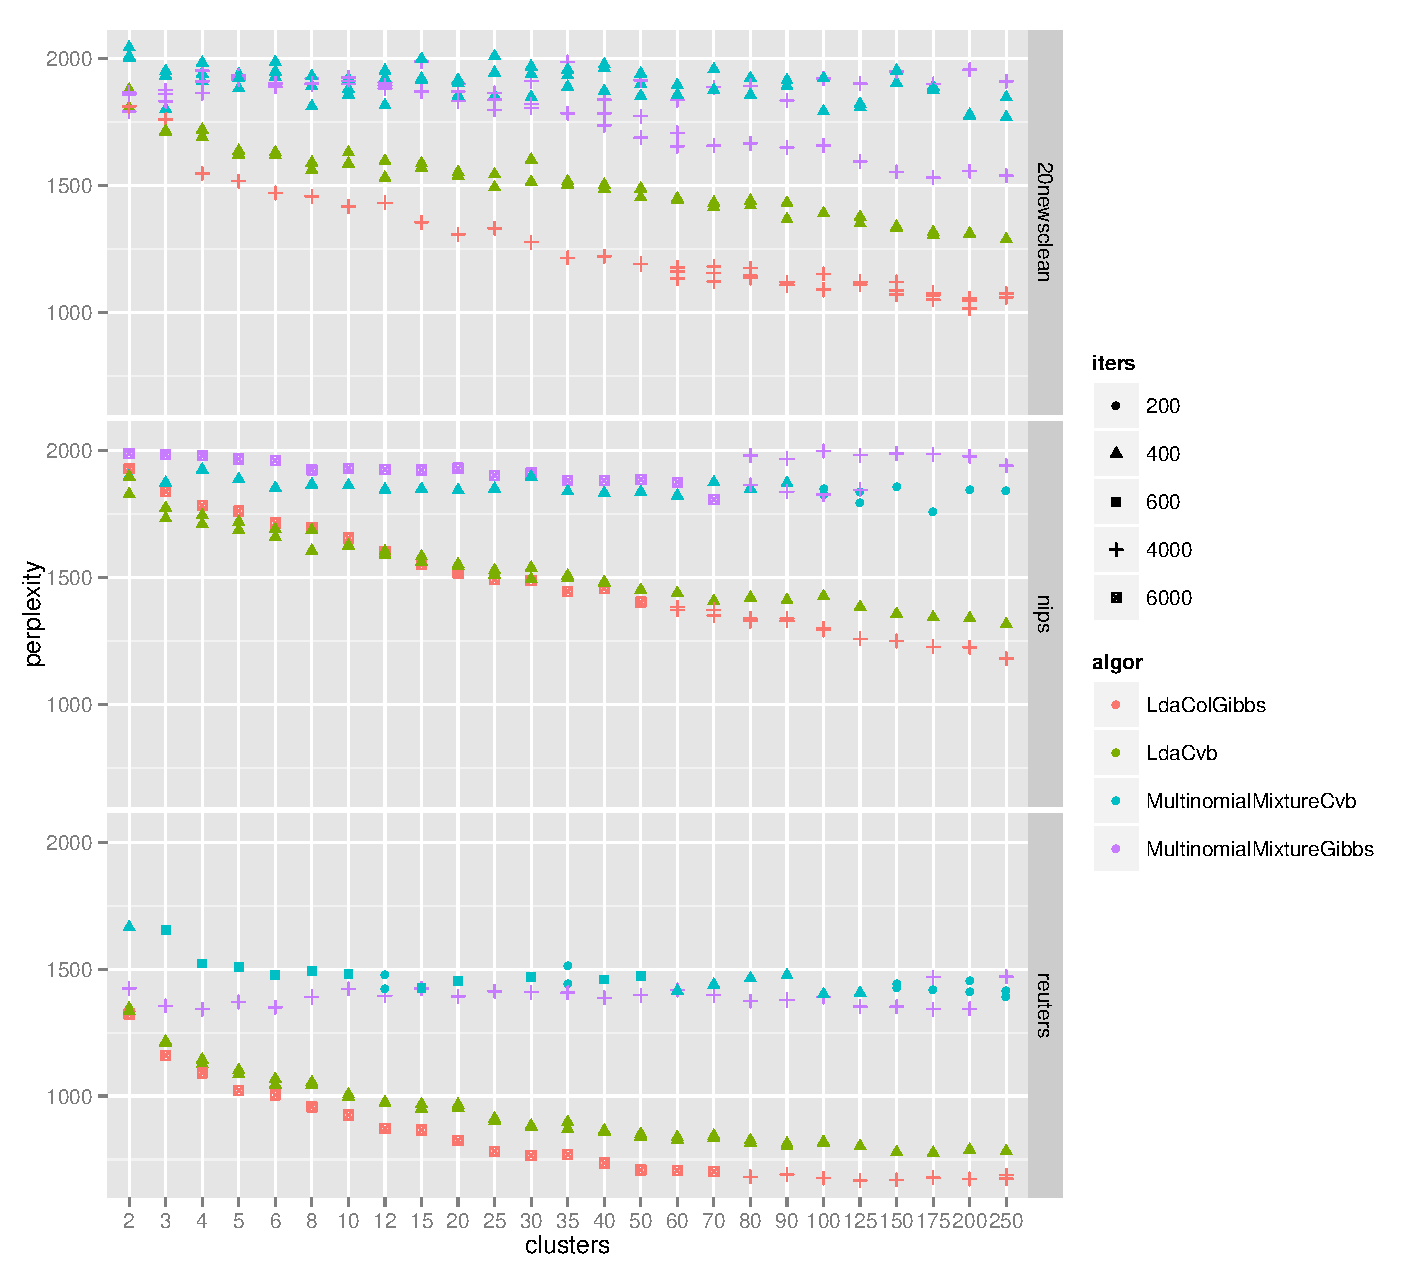
\includegraphics[width=0.9\textwidth]{plots/results-2013-03-18.pdf}
  \caption{Perplexity results for LDA and a mixture of multinomials ("MoM") implemented using Gibbs sampler and EM in the case of the mixture, and collapsed variational inference in the case of LDA. The three datasets are Reuters, NIPS, and four distinct newsgroups from the 20News dataset. The number of iterations (including burn-in for samplers) is also shown.}
  \label{fig:nip-reuters-20news-tests}
\end{figure}

\subsubsection*{Scaling to Large Datasets}
The issue of how to scale LDA to large datasets has been actively researched. With regard to variational methods, one of the earliest approaches was the Online variatinal LDA of \cite{Hoffman2010} which uses stochastic gradient descent\cite{Bottou2004}\cite{Bottou2008}, estimating the ``local" document-level topic assignments in the usual way, a document at a time\footnote{In practice ``mini-batches" of documents are used to minimise the variance}, using those estimates to update counts of topic-word assignments, and then using these derived counts to update the ``global" matrix of topic-specific vocabularies, using a a natural gradient step (which is the same as the standard update in the batch algorithm).

This was further improved in \cite{Mimno2012a} by using a Gibbs sampler in the ``local" step, which unlike the variational approach led to sparse estimate of the topic distributions, particularly for large topic counts, which in turn meant that sparse computations could be used to update the vocabulary.

This general approach of stochastic gradient descent, with ``local" and ``global" parameters has been described in some depth, for the case of the exponential family, in \cite{Hoffman2012}; however approach cannot be applied to LDA/CVB, as there is no clear separation between ``local" and ``global" variables, and moreover, to determine the new distribution $q(\zdnk)$ one requires the previous mean of that distribution to estimate terms such as $\ex{n_{dk\cdot}^{\setminus dn}}{\hat{q}}$, which one clearly cannot do with massive datasets. In \cite{Boyles2013} a variant of LDA/CVB0 is presented where one does not subtract the previous topic assignment, replacing terms like $\ex{n_{dk\cdot}^{\setminus dn}}{\hat{q}}$ with $\ex{n_{dk\cdot}}{\hat{q}}$. Instead the counts are assumed to be random variable, with gradient-style updates are used to update them in a method similar to online EM\cite{Cappe2009}, which should converge to the true counts, from which the true parameters can be derived. 

This reduces the memory requirements of LDA/CVB0 to those of LDA with a collapsed Gibbs sampler, which are still more onerous than the online variants of LDA/VB discussed heretofore. 

%\fixme{Need to read Sparse Online Topic Models\cite{Zhang2013}}

Significant effort has also been expended on making Gibbs sampling scale to large datasets. Many of these algorithmic improvements are described in \cite{Yao2009}. The most notable is to re-write the sampling distribution as

\newcommand \nodn { { ^{\setminus dn } } }

\begin{align}
\begin{split}
p(z_dn = k | \vv{z}_{d}^{\setminus dn}, w_{dn}=t) & \propto \frac{\alpha_k \beta_t}{n_{\cdot k \cdot}\nodn + \sum_v \beta_v} \\
& + n_{dk\cdot}\nodn \frac{n_{\cdot kt}\nodn + \beta_t}{n_{\cdot k \cdot}\nodn + \sum_v \beta_v} \\
& + \frac{n_{dk\cdot}\nodn n_{d\cdot t}\nodn}{n_{\cdot k \cdot}\nodn + \sum_v \beta_v}
\end{split}
\end{align}
While ostensibly more complicated, the second and third summands are sparse, and can be stored efficiently, while the first term, which is dense, is trivially changed after each update as only the denominator changes. In addition there are further purely algorithmic improvements are described in the paper, with the resulting ``SparseLDA" algorithm converging at more than ten times the speed of the standard collapsed sampler, and twice the speed of ``Fast LDA"\cite{Porteous2008}, which instead focussed on avoiding calculating all K posterior topic probabilities for each token when sampling.

%\fixme{See also Fast collapsed gibbs sampling for latent dirichlet allocation. In Proceedings of the ACM SIGKDD International Conference on Knowledge Discovery and Data Mining, pages 569–577, 2008.}

To extend this to hundreds of millions of documents, a distributed Gibbs sampler is described in\cite{Newman2009}. The setting is a Hadoop cluster, where the set of $D$ documents is paritioned into $M$ disjoint subsets, each of size $D_m$, each stored on one of $M$ machines. For the purposes of illustration, $M$ can be of the order of 1,000. A further restriction is that due to the fact that networks are much slower than CPUs, and that $2^M$ such connections exist, it is not feasible for machines to communicate with each other. Therefore the problem is how to meaningfully infer topics from the whole dataset, through machines which can only see a subset of it, albeit one which may contain 100,000 documents.

Uncollapsed Gibbs samplers can be trivially implemented in this setting, as topic assignments are conditionally independent given $\thd$ and $\pk$, so one can distributed the task of estimating $z_{dn} | \thd, \Phi$ across all machines, then use those counts in a consolidation step to update $\Theta$ and $\Phi$. However uncollapsed Gibbs samplers typically exhibit poor mixing, so it is preferable to implement a distributed, collapsed Gibbs sampler. In the map-reduce framework, estimations of $\vv{z}_d$ for all documents across many machines is the ``map" step, and the consolidation of these counts and their use in updating $\Theta$ and $\Phi$ is the reduce step.

The three sufficient statistics of a collapsed Gibbs sampler are the counts $n_{dk\cdot}$, $n_{\cdot k \cdot}$ and $n_{\cdot k t}$. A machine $m$ will know the first for the documents it stores, but will not be aware of the other two. One approach, AD-LDA, simply ignores this. At the start of each iteration, the full counts $n_{dkt}$ are broadcast to all machines, and then they proceed, using their local copies of these counts, to draw samples and so create updated counts (the ``map" step). These are then summed together at the end of the iteration (the ``reduce" step), ready for the start of the next. The intuition behind this approximation is that due to the large number of words, the number of word-topics changed by other machines $m' \neq m$ in a single iteration will have a negligible effect on the probabilities of topic assignment on machine $m$, and so the presence of such ``stale" counts on a machine $m$ disconnected from all machines $m' \neq m$ will be negligible.

A second way of thinking about this approximate model is that each machine has its own noisy sample of the topic-word counts sampled from some global distribution, which leads to naturally leads to the idea of hierarchical model. In such a model each machine's topic-specific vocabulary distributions are sampled from global topic-specific vocabularies, such that topic-assignments can be considered conditionally independent given these global vocabularies.
\begin{align}
\alpha^{(m)} & \sim \gam{a}{b} &
\vv{\theta}_d^{(m)} & \sim \dir{\alpha^{(m)}} &
\vv{\psi}_k^{(m)} & \sim \dir{\gamma} \\
\beta_k & \sim \gam{c}{d} &
z_{dn}^{(m)} & \sim \muln{\vv{\theta}_d^{(m)}}{1} &
\vv{\phi}_k^{(m)} & \sim \dir{\beta_k \vv{\psi}_k} \\
& &
& &
w_{dn}^{(m)} & \sim \muln{\vv{\phi}_{z_{dn}^{(m)}}^{(m)}}{1}
\end{align}

This approach defines a valid probabilistic model which can be decomposed across machines, however there remains the final issue of identifiability amongst topics: i.e. that topic \#1 on one machine may correspond to a distribution with index \#7, say, on another machine. A number of approaches were explored to address this. The first was simply to ignore it, to assume that topic \#1 referred to the same distribution across all machines. In practice, it was reported, this worked, as topics gradually aligned. Another approach, which converged much faster, was a greedy strategy where one machine's topics were considered the gold standard, and each subsequent machine's topics were matched to those topics using KL-divergence. Where no acceptably close match occurred, a new topic was created, so that $K$ could change between runs. 

In practice, the reported convergence and predictive likelihood was broadly similar between the approximate and hierarchical distributed samplers using the same reconciliation strategy. Both models still showed worse convergence, on small datasets, than the non-distributed batch model however.

To address this, a different approach was employed in \cite{Smola2010}. The context, once again, is a Hadoop cluster where inter-machine communication is infeasible. However a ``blackboard" server storing the sufficient statistics in a high-speed in-memory database\footnote{In this case ``Memcache"} was added to this cluster. At each iteration, for each document, each machine queried the blackboard for the latest counts $n_{\cdot k \cdot}$ and $n_{\cdot k t}$, and then proceeded to assign topics to each token in the document, finally transmitting the updated counts when all the current documents tokens had been assigned topics. This is inherently approximate -- strictly speaking counts should be queried and updated when processing every individual token, however this would mean that the time taken to process each token was the time of a round-trip across the network to the blackboard server.

The advantages of this model is that all machines can iterate to convergence independently, instead of pausing at the end of each iteration to reconcile counts. Further, by sharing counts in near real-time, the indentifiability problem is avoided. Moreover, the blackboard ``server" can in fact be composed of several servers to avoid network contention for a single machine. Each server holds a subset of counts of all possible topic-word pairs (their experiments involved corpora with vocabularies of $10^6$ words). While only guaranteeing eventual consistency in the presence of a failing node: assuming all nodes remain active for the duration of the run, all reads from a MemCache cluster should remain consistent. 

With respect to large-scale inference among correlated topic models, the most significant contribution has been\cite{Chen2013}, where batch and parallel Gibbs samplers were derived for CTM. In the batch case, the  vocabulary was collapsed out and topic-assignments for each word were drawn in the usual way from a document-level distribution. Given the topic assignments, inferring the hyperparameters of the Gaussian prior is equivalent to logistic regression. However by augmenting this likelihood with an auxiliary variable $\lambda_{dk}$ such that
\begin{align}
p(\eta_{dk} | \vv{\eta}_{d\setminus k}) & = \frac{(e^{\rho_{dk}})^{n_{dk\cdot}}}{(1 + e^{\rho_{dk}})^{n_{d\cdot\cdot}}} \qquad\qquad\qquad\text{where }\rho_{dk} = \eta_{dk} - \ln\left(\sum_{j \neq k} \eta_{dj}\right) \\
&= \frac{1}{2^{n_{d\cdot\cdot}}}
e^{\kappa_{dk} \rho_{dk}}
\int_0^\infty e^{-\halve{\lambda_{dk} (\rho_{dk})^2}} p(\lambda_{dk}|n_{d\cdot\cdot},0) d\lambda_{dk} 
\end{align}
where $\kappa_{dk} = n_{dk\cdot} - \halve{n_{d\cdot\cdot}}$ and $\lambda_{dk}$ has a Polygamma distribution, they were able to derive an exact Gibbs step, instead of resorting to the more usual approach of rejection sampling with some proposal distribution. Finally, a Normal/Inverse-Wishart prior was used for the topic mean and covariance.

As with the distributed Gibbs LDA algorithm of \cite{Newman2009}, by employing hierarchical priors, it is possible to distribute this across several machines. Specifically the topic strength vectors $\vv{\eta}_d$ for each document $d$ are conditionally independent of one another given the $\mathcal{NIW}\left(\vv{\mu}, \rho, \kappa, \Sigma\right)$ prior. The per-token topic assignments need the global $n_{\cdot k t}$ counts, and these are made available via a blackboard server similar to \cite{Smola2010}. As with \cite{Yao2009} careful attention was taken to exploit sparsity when implementing the posterior sampler over topic assignments. Finally an approximate sampling algorithm for the PolyGamma distribution was employed to speed the implementation further.

% ---- Gibbs optimisations ----




% ---- Other approaches ----



\bibliographystyle{plain}
\bibliography{/Users/bryanfeeney/Documents/library.bib}

\end{document}

